\documentclass[10pt]{article}
\usepackage[margin=0.7in]{geometry}
\usepackage[T1]{fontenc}
\usepackage{graphicx,booktabs,amsmath,amssymb,hyperref}
\hypersetup{hidelinks}
\setlength{\parindent}{0pt}
\setlength{\parskip}{5pt}
\begin{document}
{\LARGE Blind primitive-law review}\par
\textbf{TASK-20261027-8805a4; J-primitive-law; 2026-10-27}

\textbf{Scoped verdict: holds.} Independent derivation and affine software agree with one group event per explicit add invocation, including identity, inverse and doubling. This is a primitive software check; it attests no production execution, native count, runtime or scientific promotion.

\textbf{Observation.} The only scientific inputs were the sanitized statement and review plan. No producer implementation, native rows, old ratios, result-bearing Git history or sibling report was read. Public fixture:
\[
 E/\mathbb{F}_{383}: y^2=x^3+261x+146,\qquad P=(196,297),\quad r=181.
\]
Exact arithmetic gives discriminant $156\bmod383$, $P\in E$, $jP\ne O$ for $1\le j<181$, and $181P=O$. Separate affine addition functions use modular inversion and Fermat inversion; repeated addition supplies the answer oracle. All 513 fixed public scalars $0\ldots512$ agree in answers and counts. Seven primitive cases each invoke add once: $O+O$, $O+P$, $P+O$, $P+(-P)$, $P+P$, $P+(2P)$, and $(66,0)+(66,0)$. The latter is an on-curve order-two edge case outside $\langle P\rangle$.

\textbf{Derivation.} For noninverse finite inputs, the chord or tangent slope gives $(m^2-x_1-x_2,\;m(x_1-x_3)-y_1)$ modulo $p$. All affine branches still count one invocation. For $k\ge0$, let $L=\operatorname{bitlength}(k)$, $L(0)=0$, and $w=\operatorname{popcount}(k)$. The exact handout loop calls the accumulator add $w$ times and the base double after every bit except the last:
\[
 D=\max(L-1,0)\quad\hbox{base-doubling invocations},\qquad G=w+D.
\]
\begin{center}
\begin{tabular}{rrrrl}\toprule
$k$&$w$&$D$&$G$&$kP$\\\midrule
0&0&0&0&$O$\\
1&1&0&1&$(196,297)$\\
2&1&1&2&$(359,269)$\\
3&2&1&3&$(141,93)$\\
180&4&7&11&$(196,86)$\\
181&5&7&12&$O$\\
182&5&7&12&$P$\\
331&5&8&13&$(262,200)$\\
362&5&8&13&$O$\\\bottomrule
\end{tabular}
\end{center}
The same counts hold for base $O$ at $k=0,1,r,r+1,2r$; every answer is $O$. There is no scalar reduction or identity shortcut in the handout loop.

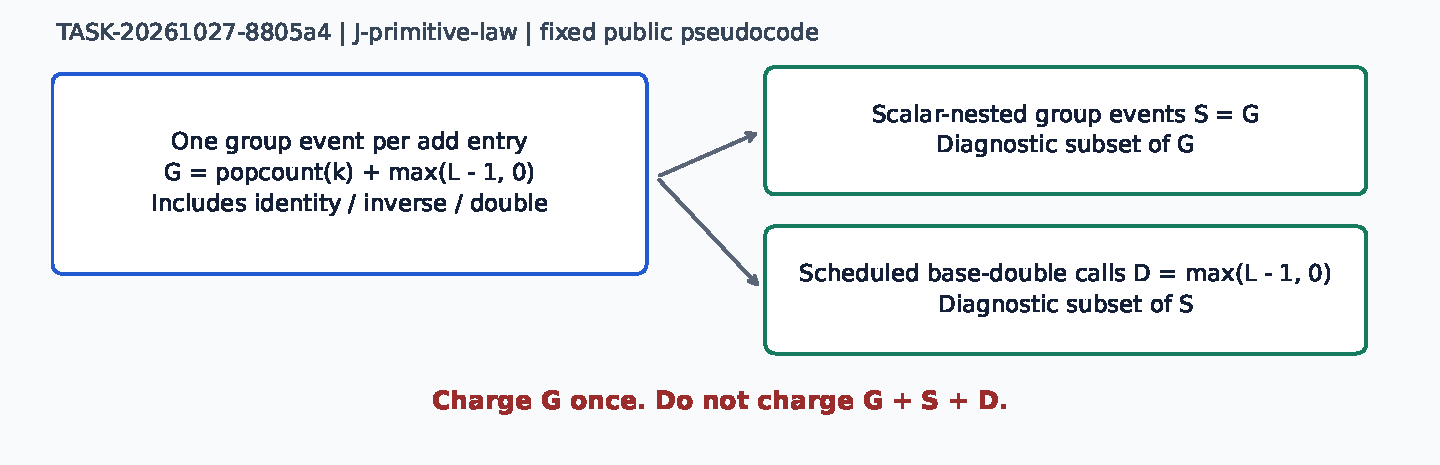
\includegraphics[width=\linewidth]{diagram.pdf}

\newpage
\textbf{Diagnostic semantics.} Scalar method entry is a diagnostic (one even for $k=0$). Scalar-nested group events satisfy $S=G$ in this scalar-only routine. Scheduled base doubles are a subset of these events. Adding $G+S+D$ charges the same calls repeatedly. Affine tangent branches are a different label: at $k=331$, $D=8$ but nine calls enter the tangent branch because an accumulator add also has equal inputs. No unspecified production diagnostic is assumed to have either meaning.

\textbf{Control.} At $k=181$, the exact group count is 12 and the scalar answer is $O$. The correct answer/count pair passes. The same correct answer with advertised count 13 fails the cost check while passing the witness check. A wrong answer $P$ with count 12 fails the witness check. Correct scalar equations alone therefore do not certify counts. No breaking artifact against the specified primitive law was found; the actual mutation and traces are retained.

\textbf{Evidence bindings.} All files below are local to this task directory unless otherwise identified. The JSON record contains full SHA-256 bindings.
\begin{itemize}
\item \texttt{independent\_arithmetic.py}: independently written affine check, exact binary loop, entry-event log and assertions.
\item \texttt{predicted-counts.json}: analytical predictions, observed software events for selected cases, finite check summary and known-false control.
\item \texttt{review.json}, \texttt{read-attestation.yaml}: scope, verdict, exact inputs read, limits and requested inference policy.
\item Batch scientific sources: \texttt{blind-packet/statement.json} (SHA-256 prefix \texttt{44e63aa2d557}) and \texttt{review-plan.yaml} (\texttt{3b789c014501}).
\item \texttt{report.md} is the fuller narrative; \texttt{diagram.py} generates the local SVG/PDF. This PDF was rendered from \texttt{report.tex}.
\end{itemize}

\textbf{Limitations.} This checks only J-primitive-law, with mathematical definitions and the fixed sanitized handout. The public software check is not a new experiment, native benchmark, private-input exercise or full-algorithm replay. The event observer and formula see this independent program; they cannot attest historical native execution or production coverage. The repeated-add oracle shares elementary affine definitions and is not a formal proof. Group invocations are not field-operation, memory, CPU or time costs. Negative scalars, different loops, reduced-scalar APIs, precomputation and native diagnostics require separate specifications.

External literature and old research were not consulted because the blind handout restricts scientific inputs. There is no novelty or prior-art claim. Repository policy/workflow sources are separately listed in the read attestation. No canonical graph was read or changed, because that exceeds the blind scope; this local diagram explains only the primitive accounting. The parent's clarification added base $O$ and explicit $r$ boundaries without lifting blindness.

\textbf{Provenance and next action.} Requested role/policy: reviewer, review-adversarial, xhigh. Serving model and probe verification: unknown/unverified; no backend attestation is claimed. No official status, hypothesis or claim qualification changes. Archive task TASK-20261027-598d0d owns commit/push; this reviewer performs neither. The Coordinator may compare the predicted law with other independently assigned joints while retaining native-execution and runtime gaps.
\end{document}
